
%(BEGIN_QUESTION)
% Copyright 2014, Tony R. Kuphaldt, released under the Creative Commons Attribution License (v 1.0)
% This means you may do almost anything with this work of mine, so long as you give me proper credit

Anta at måleren i denne Wheatstone-bro-kretsen står ``i endestopp'' selv når RTD-en er ved 0$^{o}$ C (når broen skulle vært balansert), med polaritet over voltmeterterminalene som vist:

$$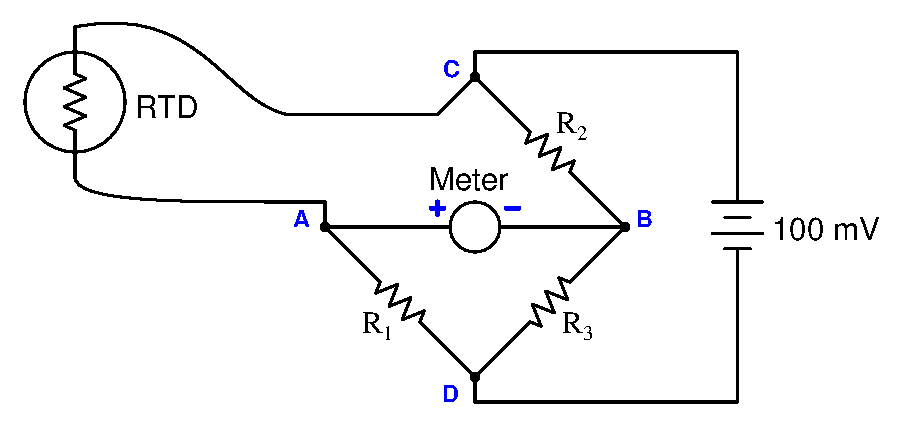
\includegraphics[width=15.5cm]{i00943x01.eps}$$

Vurder sannsynligheten for hver angitt feil i kretsen. Se på én feil om gangen (ingen samtidige feil), og avgjør om den alene kan forklare {\it alle} målinger og symptomer.

% No blank lines allowed between lines of an \halign structure!
% I use comments (%) instead, so that TeX doesn't choke.

$$\vbox{\offinterlineskip
\halign{\strut
\vrule \quad\hfil # \ \hfil & 
\vrule \quad\hfil # \ \hfil & 
\vrule \quad\hfil # \ \hfil \vrule \cr
\noalign{\hrule}
%
% First row
{\bf Feil} & {\bf Mulig} & {\bf Umulig} \cr
%
\noalign{\hrule}
%
% Another row
$R_1$ feilet åpen &  &  \cr
%
\noalign{\hrule}
%
% Another row
$R_2$ feilet åpen &  &  \cr
%
\noalign{\hrule}
%
% Another row
$R_3$ feilet åpen &  &  \cr
%
\noalign{\hrule}
%
% Another row
RTD feilet åpen &  &  \cr
%
\noalign{\hrule}
%
% Another row
$R_1$ feilet kortsluttet &  &  \cr
%
\noalign{\hrule}
%
% Another row
$R_2$ feilet kortsluttet &  &  \cr
%
\noalign{\hrule}
%
% Another row
$R_3$ feilet kortsluttet &  &  \cr
%
\noalign{\hrule}
%
% Another row
RTD feilet kortsluttet &  &  \cr
%
\noalign{\hrule}
} % End of \halign 
}$$ % End of \vbox

\underbar{file i00943}
%(END_QUESTION)





%(BEGIN_ANSWER)

% No blank lines allowed between lines of an \halign structure!
% I use comments (%) instead, so that TeX doesn't choke.

$$\vbox{\offinterlineskip
\halign{\strut
\vrule \quad\hfil # \ \hfil & 
\vrule \quad\hfil # \ \hfil & 
\vrule \quad\hfil # \ \hfil \vrule \cr
\noalign{\hrule}
%
% First row
{\bf Feil} & {\bf Mulig} & {\bf Umulig} \cr
%
\noalign{\hrule}
%
% Another row
$R_1$ feilet åpen & $\surd$ &  \cr
%
\noalign{\hrule}
%
% Another row
$R_2$ feilet åpen & $\surd$ &  \cr
%
\noalign{\hrule}
%
% Another row
$R_3$ feilet åpen &  & $\surd$ \cr
%
\noalign{\hrule}
%
% Another row
RTD feilet åpen &  & $\surd$ \cr
%
\noalign{\hrule}
%
% Another row
$R_1$ feilet kortsluttet &  & $\surd$ \cr
%
\noalign{\hrule}
%
% Another row
$R_2$ feilet kortsluttet &  & $\surd$ \cr
%
\noalign{\hrule}
%
% Another row
$R_3$ feilet kortsluttet & $\surd$ &  \cr
%
\noalign{\hrule}
%
% Another row
RTD feilet kortsluttet & $\surd$ &  \cr
%
\noalign{\hrule}
} % End of \halign 
}$$ % End of \vbox


%(END_ANSWER)





%(BEGIN_NOTES)

{\bf Denne oppgaven er ment kun for eksamen, ikke for arbeidsark!}.

%(END_NOTES)

